Trong mối quan hệ bất đối xứng, một bối cảnh giới hạn có sự phụ thuộc vào một bối cảnh giới hạn khác. Mối quan hệ này được mô tả bằng cách gán vai trò cho bối cảnh giới hạn:

\begin{itemize}

    \item \textbf{Bối cảnh giới hạn thượng nguồn (Upstream):}
          \begin{itemize}


              \item     Bối cảnh giới hạn cung cấp cho bối cảnh giới hạn khác.
              \item Ký hiệu:      U
          \end{itemize}

    \item \textbf{Bối cảnh giới hạn hạ lưu (Downstream):}
          \begin{itemize}
              \item    Bối cảnh giới hạn phụ thuộc vào bối cảnh giới hạn khác.
              \item Ký hiệu:     D
          \end{itemize}


\end{itemize}

\begin{example} Mối quan hệ bất đối xứng giữa      bối cảnh giới hạn A và     bối cảnh giới hạn B.
    \begin{itemize}
        \item      Bối cảnh giới hạn  A ràng buộc với      bối cảnh giới hạn  B

        \item      Bối cảnh giới hạn  A đóng vai trò là bối cảnh giới hạn hạ lưu (Downstream)

        \item      Bối cảnh giới hạn  B đóng vai trò là bối cảnh giới hạn thượng nguồn (Upstream)

        \item      Bối cảnh giới hạn    A có kiến thức về các mô hình trong bối cảnh giới hạn B

        \item      Bối cảnh giới hạn  B không có bất kỳ kiến thức nào về mô hình trong bối cảnh giới hạn A
    \end{itemize}

    \begin{figure}[H]

        \centering

        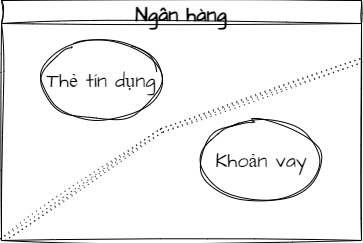
\includegraphics[scale = 0.5]{pictures/mo_hinh_rieng_biet_separate_ways/main.drawio.png}

        \caption{Ví dụ  mối quan hệ bất đối xứng }

    \end{figure}
\end{example}



%! $VD: A Downstream (D) - B Upstream (U) - - >



